\section{Implementation}
\label{sec:implementation}

\subsection{System Design}

Backscattered light from an object hit by a laser, like a speckle pattern, is typically very low in intensity. How low depends on the situation.

The light intensity $I_b$ at a distance $d$ is proportional to the laser power and decays quadratically with distance and can be calculated using a simplified model:

\begin{equation}
I_b = \frac{P \cdot \rho}{2\pi d^2},
\end{equation}
where:
\begin{itemize}
\item $P$ is the power of the incident laser beam, measured in watts (W),
\item $\rho$ is the reflectivity of the surface (unitless),
\item $d$ is the distance from the scattering surface to the photodiode, measured in meters (m).
\end{itemize}


\subsection{How much current?}
A photodiode converts the backscattered light intensity into current:
\begin{equation}
I_{\text{photo}} = I_b \cdot A_{\text{PD}} \cdot R,
\end{equation}
where:
\begin{itemize}
\item $I_b$ is the incident intensity at distance $d$ \text{(W/mm\textsuperscript{2})},
\item $A_{\text{PD}}$ is the area of the photodiode \text{(mm\textsuperscript{2})},
\item $R$ is the photodiode responsivity \text{(A/W)}.
\end{itemize}
Using typical values like $R = 0.5\text{A/W}$, $A_{\text{PD}} = 2\text{ mm}^2$, $P = 1\text{ mW}$ and $d = 0.3\text{ m}$ we are left with tiny photocurrents in the $500\text{ pA}$ range!

To be certain, we conduct a small set of experiments (setup is shown in Figure \ref{fig:cam1}) to measure the current produced by a photodiode exposed to incident laser speckle pattern.

A typical store-bought class 1 red laser pointer has an output power under 0.5mW. 
Using this laser pointer and the Thorlabs PDA36A2 photodetector (with a photodiode area: $A_{\text{PD}} = 13\text{ mm}^2$ and same $d$ as above), we observe ~13 ~nA of current.
This means that we need to at least be able to measure currents on this order of magnitude for class 1 lasers at ~30 ~cm distance.


\subsection{How big a photodiode?}
Can we test if a photodiode of a given size can be sensitive to a speckle pattern in motion? Recall that the sensor must be smaller than the speckle size in order to resolve speckle motion. Using the formula for mean speckle size, assuming a red laser at 650 ~nm and 30 ~cm distance, we find the resulting mean size to be around 100 ~um. This is smaller than common photodiodes. We make the assumption - based on observations of real speckle patterns - that the variance in size is large. That means that some speckles will be on the order of a common small photodiode ($1\text{ mm}^2$), meaning that we will be able to sense a variance in intensity when speckles pass over the photodiode.

To validate this assumption, we masked the detector with a 0.9mm x 0.9mm pinhole (poked a hole, then measured it) on copper tape to cover the aperture of the detector (inspired by \cite{veber2011laserMASK}). 
We set the surface in motion and observed the output on a multimeter as well as on camera. As the speckle oscillated on camera, so did the multimeter output.

With this, we find the most sensitive, small, low cost photodiode on Digikey: the VEMD2704 by Vishay with an area of $1.5\text{ mm}^2$.

\subsection{How many photodiodes?}
We know we can detect the speckle pattern translation with 1 photodiode. And while we can calculate the mean speckle size, we have no grasp of its variance with just one photodiode. If we arrange multiple photodiodes in a grid, some of them will see darker spots and some will see lighter spots. This means that given a grid of photodiodes, we can detect the global change in speckle pattern variance. 

We use the Raspberry Pi HQ camera sensor to determine the spacing and size of the grid experimentally.

We make the following observations:
\begin{itemize}
  
  \item A CMOS sensor pixel is a photodiode and has as determined size.
  \item We can emulate the output of a larger photodiode by integrating over all pixels over the same area as the larger photodiode.
  \item The sensor area of the RPI camera is large enough to accommodate 9 VEMD2704 photodiodes (see Figure \ref{fig:emulated2}).
\end{itemize}

Using this knowledge, we record a video of a speckle pattern in motion and cut out the pixels corresponding to a grid of areas the same sizes as the VEMD2704.
We establish that an algorithm similar to the one used by Streli et al \cite{structured-light-speckle} can be used to combine the outputs of the photodiodes in order to create a 1d motion signal.
Figure \ref{fig:emulated2} shows the resulting 1d signal of motion (essentially speckle pattern variance). The section on Signal Processing discusses this in detail.

In fact, in the camera experiments we only simulated a horizontal grid of 3 VEMD2704 photodiodes. Using a 3x3 grid would theoretically allow direction sensing, but this was not tested. A 3x3 grid also increases SNR as we have more samples to compute the speckle variance.

\subsection{Hardware Implementation}
We want a simple and cost effective solution, to amplify and digitize the photodiode signals, that is flexible enough for experimentation.
A single amplifier stage is chosen that is directly coupled, through an antialiasing filter, to an analog to digital converter (ADC). 

Photodiodes are commonly amplified using a transimpedance amplifier (TIA), or a current to voltage amplifier. Although alternative options exist, such as current integrators like the DDC118, they require more complex setups and control.

The TIA current to voltage gain and bandwidth is defined by the the feedback path.

\begin{equation}
V_{\text{out}} = R_f \cdot I_{\text{in}},
\end{equation}
where:
\begin{itemize}
\item $V_{\text{out}}$ is the output voltage (V)
\item $R_f$ is the feedback resistance ($\Omega$)
\item $I_{\text{in}}$ is the input current (A)
\end{itemize}

\begin{equation}
f_{-3\text{dB}} = \frac{1}{2\pi R_f C_f},
\end{equation}
where:
\begin{itemize}
\item $f_{-3\text{dB}}$ is the -3dB bandwidth (Hz)
\item $R_f$ is the feedback resistance ($\Omega$)
\item $C_f$ is the feedback capacitance (F)
\end{itemize}

We want a gain that supports a good range of AC and DC photocurrent. We assume that we will have 1nA peak-to-peak AC induced by a IR speckle pattern in motion. No analog DC rejection is performed, to keep things simple, so we must account for microamps of potential DC photocurrent. If we use a 100 MOhm feedback resistor, we can achieve 100 mV AC output. In order to not saturate the opamp with DC current, filtering the input light with an IR bandpass filter is a must. For indoor purposes, there is practically no IR content in typical LED office lighting, though rooms with lots of natural light would still pose problems. From the power vs spectrum graphs of white LEDs, we deduce that at 850nm the VEMD2704 would output around 10nA of current - not saturating our opamp.

The bandpass filter is chosen to be IR at 850nm as that is conveniently where silicon photodiodes are most efficient. Lasers at 850nm are also very common.
 
To maximise possible bandwidth, we choose a minimal amount of feedback capacitance, which is just the stray capacitance coming from the feedback resistor (0.2 pF). Using the above formula, the amplifier bandwidth is 7.9 kHz. 

We now use the feedback path and photodiode parameters in Formula 10 of \cite{TIABW}, to calculate a required GBW (gain bandwidth product) for guaranteed amplifier stability. We find that we must choose an operational amplifier with more than 1110 kHz of GBW.

For a simple experimental setup, we want to use a Raspberry Pi for data processing, recording and visualisation. Many relatively high speed and low cost ADCs exist for the Raspberry Pi, that are easily read out via Python. The data rates are on the order of 1-10kSPS per channel.

We test two ADCs in this project:
\begin{itemize}
  \item Waveshare High-Precision AD HAT (ADS1263): 10 channel mux, 1 ADC with 32-Bit resolution, 38400 SPS (total).
  \item Digilent MCC128: 8 channel mux, 1 ADC with 16-bit resolution, 100 kSPS (total).
\end{itemize}
Both are multichannel ADCs that use a multiplexer to switch between all channels. 

The first ADC was unable to sample at high enough frequencies. The channel switching is controlled via SPI, making it challenging to manage the switching delay and the effective sample rate. This mux also produced a significant amount of noise, even with filtering, which was noted in several GitHub issues reported by users. Only a low sample rate of around 200 Hz was achieved.

The second ADC was then tested, featuring a higher sample rate and advertised synchronous sample readout capability. Unfortunately this ADC inexplicably uses the Pi's 5V supply as its analog reference. However, this is very noisy, with peak-to-peak noise in the millivolt range. To mitigate this issue, a bench power supply was used to power the ADC externally. Stable sampling frequency of 4kHz per channel could be achieved.

We limit the bandwidth of the amplifier stage to 1.5~kHz (half the sample rate of the first ADC) with an RC low pass filter. This is done to prevent aliasing noise in the ADC.

We devise a system block diagram in Figure \ref{fig:block}.

\begin{figure}[t]
  \centering
  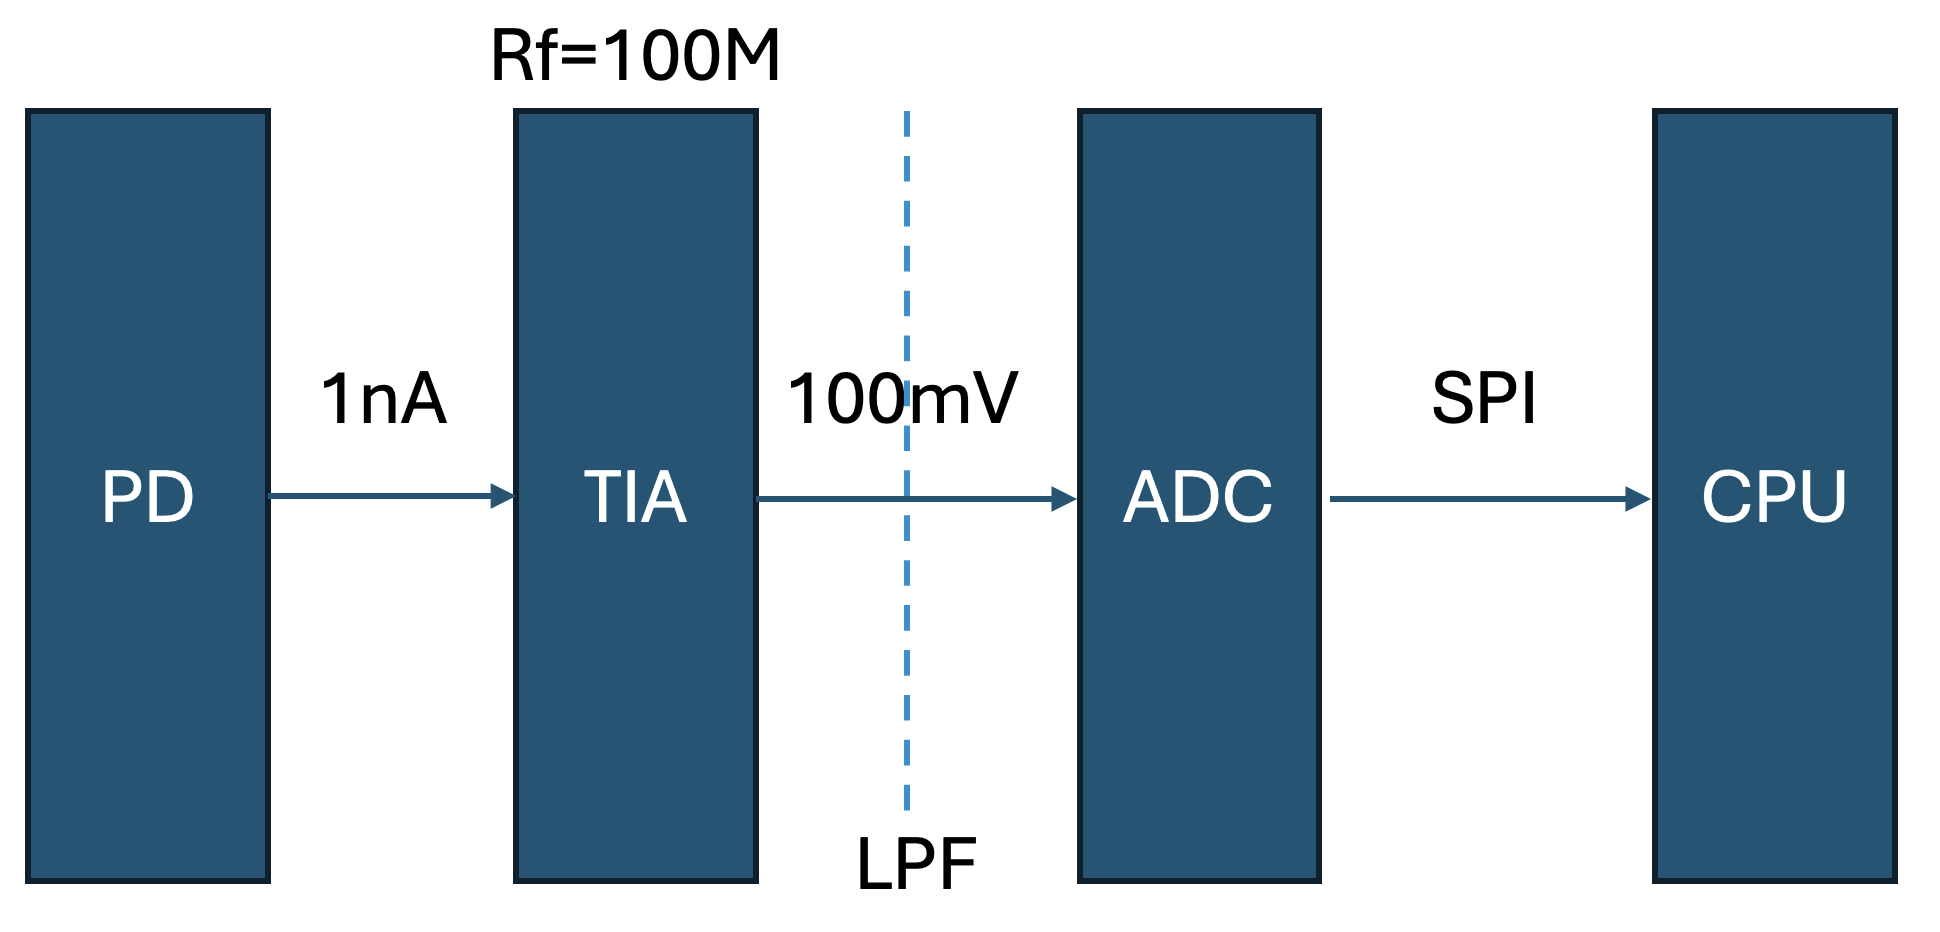
\includegraphics[width=\widthnarrow]{figures/impl/block_diagram.png}
  \caption{Block diagram}
  \label{fig:block}
\end{figure}

The essential requirements for the op-amps include:
\begin{itemize}
  \item A minimum of two op-amps in a single package.
  \item A target price of approximately \$5 per chip.
  \item JFET input with low input bias current.
  \item Low noise, low voltage offset and low voltage offset drift.
  \item Capability to operate on a single power supply.
  \item To guarantee stability, it must have a GBW of at least 1100 kHz.
\end{itemize}

The OPA2380 fulfills these requirements and a PCB was designed and built according to the datasheet recommendations. The simplified schematic is given in Figure \ref{fig:spice}.

\begin{figure}[t]
\centering
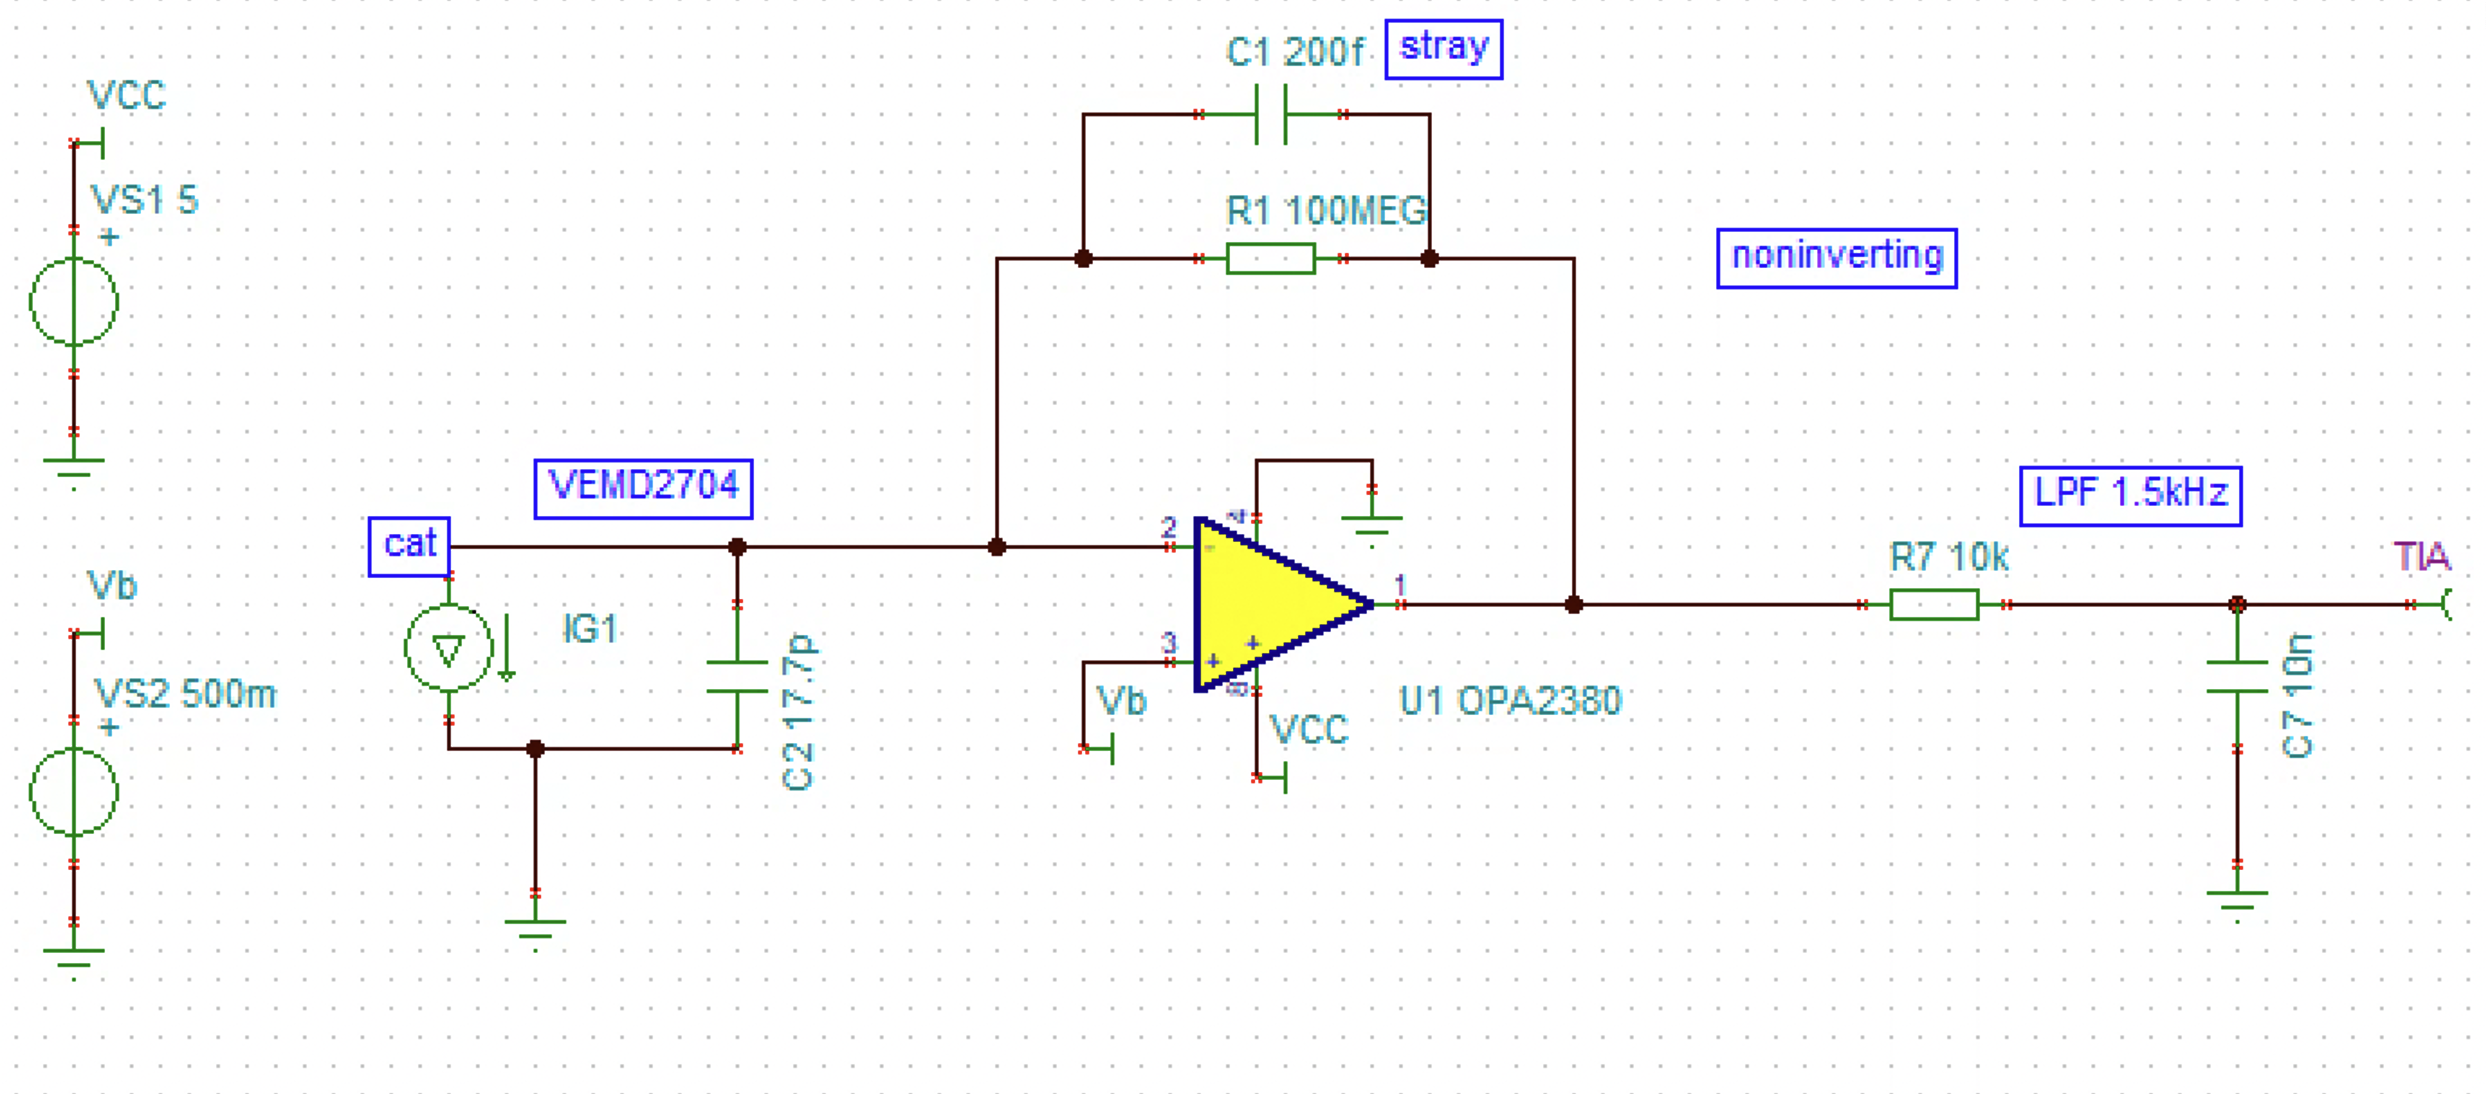
\includegraphics[width=\widthnarrow]{figures/eval/spice.png}
\caption{Amplifier schematic with equivalent photodiode (VEMD2704) and output filter.}
\label{fig:spice}
\end{figure}
      
Particular attention to leakage currents in the feedback path was taken, like the implementation of a guard ring. The guard ring is a low impedance path for any stray AC that might want to make its way into the feedback path of the amp. The PCB is shown in Figure \ref{fig:teaser} and contains a modular photodiode array with bandpass filter.


\subsection{Signal Processing}
To convert the 9-channel photodiode array readings into a single vibrometry signal, we compute the inter-channel variance, explained later on. 
First, we remove common-mode fluctuations by subtracting the instantaneous mean across all channels:

\begin{equation}
s_i(t) = r_i(t) - \frac{1}{n}\sum_{k=1}^{n} r_k(t)
\end{equation}

where $r_i(t)$ is the raw intensity reading from channel $i$ and $n=9$ is the number of channels. We then compute the inter-channel variance:

\begin{equation}
V(t) = \frac{2}{n(n-1)} \sum_{i=1}^{n-1} \sum_{j=i+1}^{n} |s_i(t) - s_j(t)|
\end{equation}

This metric quantifies the average magnitude of pairwise intensity differences between spatial channels in the instantaneous speckle pattern. 
Changes in $V(t)$ over time indicate surface motion and vibration while being robust to common-mode noise.

Raw data from the ADC was recorded and observed in real-time or processed post-capture. 
Real-time observations were conducted while simultaneously monitoring the speckle camera and the infrared (IR) camera.

\begin{figure*}[t]
  \centering
  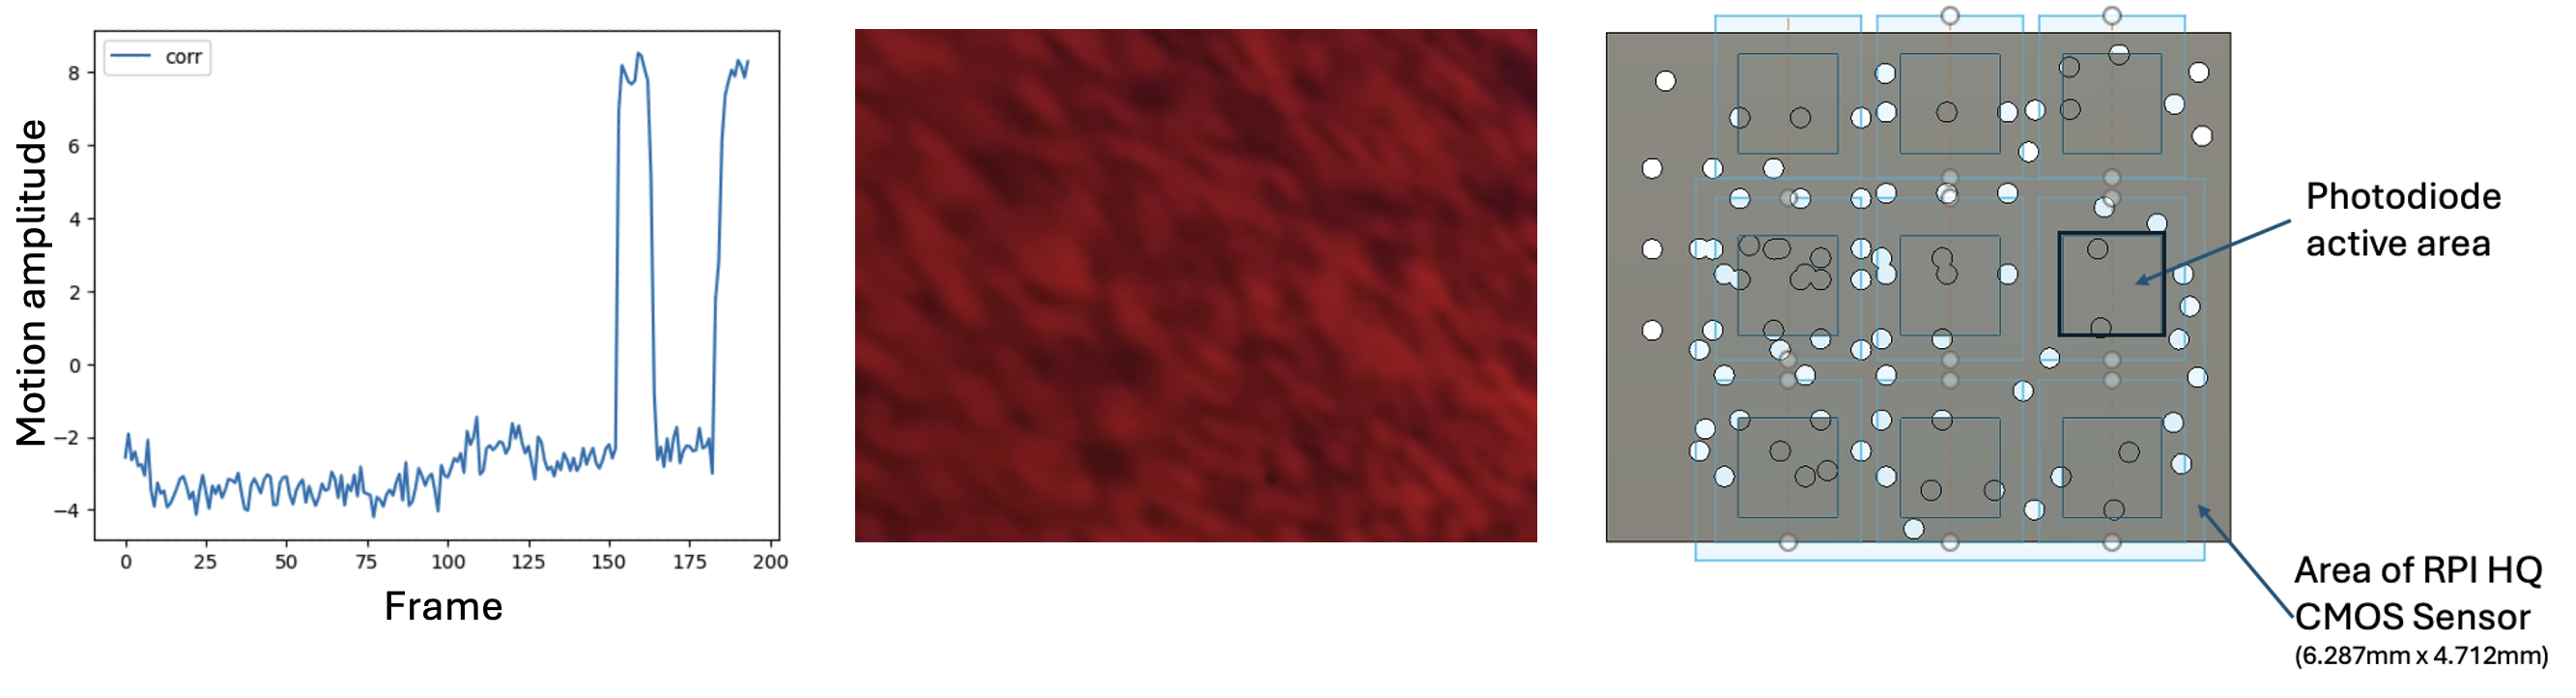
\includegraphics[width=\textwidth]{figures/impl/emulated2.png}
  \caption{Left to right: Peaks show translation of speckle pattern, signifying a change of the inter-channel variance. The speckle pattern on the camera sensor. The camera sensor with an overlayed photodiode grid.}
  \label{fig:emulated2}
\end{figure*}

\subsection{Lasers}

Several laser sources were built in different configurations as seen in Figure~\ref{fig:lasers}. 
The laser module used for the square array, circular array and single laser measurements is an 850~nm laser (VLM-850-03 by Quarton Inc.).
The Realsense D415 Depth Camera (by Intel) has a laser dot projector that can be turned on using the Realsense Viewer Software. 
To control the amount of laser dots that are output by the Realsense dot projector, an iris diaphragm (Edmund Optics 53906) is used.

Additionally, we reverse engineered the Realsense through visual inspection and found it to look very similar, if not identical, to the BELICE projector module by ams. 
To confirm this theory, we measured the laser output power with an integrating sphere on optical power meter (the Artifex OPM150) and found a similar nominal output power of 250 ~mW per module.
As a proof of concept for potential future experiments, a small driver circuit was built based on the example in the LT1800 opamp datasheet \cite{lt1800}. 